\subfloat[Assisted] {
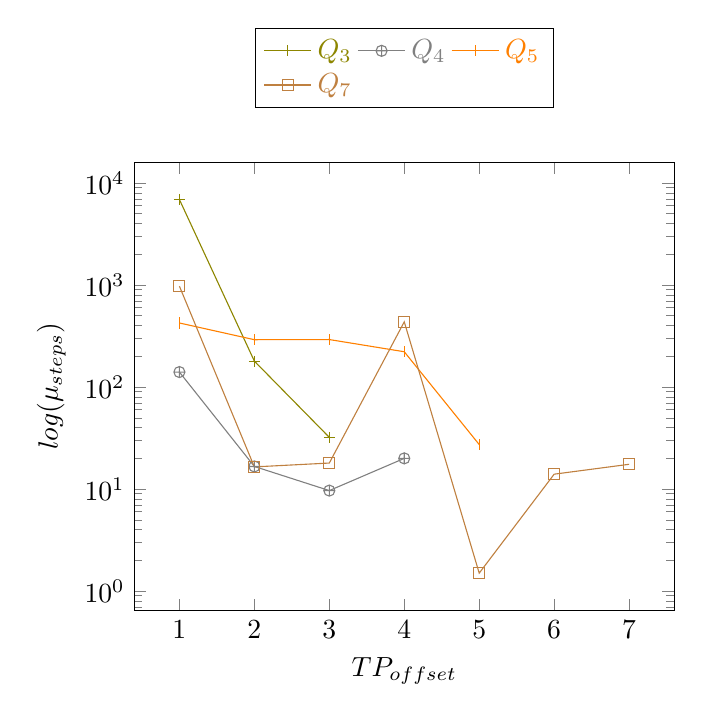
\begin{tikzpicture}\begin{semilogyaxis}[xlabel=$TP_{offset}$,
ylabel=$log(\mu_{steps})$,
  legend entries={
% [blue]$Q_2$,
   [olive]$Q_3$,
   [gray]$Q_4$,
   [orange]$Q_5$,
% [purple]$Q_6$,
   [brown]$Q_7$,
%   [pink]$Q_8$,
%   [yellow]$Q_9$,
 [black]$Q_{11}$,
% [green]$Q_{13}$,
  },
  legend columns=3,
legend style={at={(0.5,1.3)},anchor=north}]
\addplot[mark=+, style=solid, color=olive] coordinates
{ (1, 6895.0714285714275) (2, 179.71428571428572) (3, 32.14285714285714) };
\addplot[mark=oplus, style=solid, color=gray] coordinates
{ (1, 140.33333333333334) (2, 16.666666666666668) (3, 9.666666666666666) (4, 20.0) };
\addplot[mark=|, style=solid, color=orange] coordinates
{ (1, 425.0) (2, 291.33333333333337) (3, 292.33333333333337) (4, 222.0) (5, 27.333333333333336) };
\addplot[mark=square, style=solid, color=brown] coordinates
{ (1, 975.0) (2, 16.5) (3, 18.0) (4, 436.0) (5, 1.5) (6, 14.0) (7, 17.5) };
%\addplot[mark=asterix, style=solid, color=black] coordinates
%{ (1, 0.0) (2, 29.0) (3, 1.0) (4, -1.0) (5, 29.0) (6, 135.0) (7, 1.0) (8, 0.0) (9, 1281.0) (10, 1.0) (11, 28.0) };
\end{semilogyaxis}\end{tikzpicture}
}
